% Useful packages
\documentclass[12pt]{article}
\usepackage[a4paper, left=0.75in, right=0.75in, top=0.75in, bottom=0.75in]{geometry}
\usepackage{amsmath}
\usepackage{amssymb}
\usepackage{float}
\usepackage{tabularx}
\usepackage{array}
\usepackage{multirow}
\usepackage{booktabs}
\usepackage{minted}
\usepackage{xcolor}
\usepackage{enumitem}
\usepackage{hyperref}
\usepackage{graphicx}
\usepackage{longtable}
\usepackage{adjustbox}
\usepackage{textcomp}
\usepackage{subcaption}
\usepackage{mathtools}
\usepackage[nottoc,numbib]{tocbibind}

% chktex-file 13
% chktex-file 24
% chktex-file 36
% chktex-file 44

% Customizations
\definecolor{inputGray}{HTML}{f8f8f8}
\definecolor{outGray}{HTML}{dfdfdf}


\title{%
    machine learning in computational biology \\
    \Large assignment 2
    }
\author{%
    Konstantinos Konstantinidis \\
    Student number: 7115152400017
    }

\begin{document}

\maketitle

\vspace{0.5in}

\textbf{\underline{Repo:}} The repository for this assignment can be found %
here: \\
\url{https://github.com/KonsKons26/Assignment-2}

\vspace{0.5in}

% Table of contents
\tableofcontents
\clearpage



%%%%%%%%%%%%%%%%%%%%%%%%%%%%%%%%%%%%%%%%%%%%%%%%%%%%%%%%%%%%%%%%%%%%%%%%%%%%%%%%
%%%%%%%%%%%%%%%%%%%%%%%%%%%%%%%%%%%%%%%%%%%%%%%%%%%%%%%%%%%%%%%%%%%%%%%%%%%%%%%%
\section{Abstract}

In this assignment, we are tasked with classifying a dataset consisting of 512
samples of fine needle aspirate (FNA) measurements from breast masses. Each
sample is represented by 30 features, and the goal is to predict whether the
mass is malignant or benign. The dataset will be split into a training set and a
holdout set; the training set will be used to train a set of classifiers, and
the holdout set will be used to evaluate the performance of the best one using
bootstrapping.

The classifiers will be tuned using \texttt{Optuna}, a hyperparameter
optimization framework, while the features will be selected using \texttt{mRMR},
a feature selection method which minimizes the redundancy between features and
maximizes their relevance to the target class. The classifiers will be evaluated
using several metrics from the \texttt{scikit-learn} library.

The classifiers used in this assignment are:

\begin{itemize}
    \item Logistic Regression (LR) with Elastic Net regularization
    \item Gaussian Naive Bayes (GNB)
    \item Linear Discriminant Analysis (LDA)
    \item Support Vector Machine (SVM)
    \item Random Forest (RF)
    \item LightGBM (LGBM)
\end{itemize}

All models performed exceptionally well, with the best one being the
\textbf{baseline} (no feature selection) \textbf{Logistic Regression}. The
\textbf{optimal hyperparameters} for the LR classifier were:
\begin{center}
    \texttt{C = 0.067}
    $\bullet$ 
    \texttt{l1\_ratio = 0.019}
    $\bullet$ 
    \texttt{max\_iter = 9613}
\end{center}



%%%%%%%%%%%%%%%%%%%%%%%%%%%%%%%%%%%%%%%%%%%%%%%%%%%%%%%%%%%%%%%%%%%%%%%%%%%%%%%%
%%%%%%%%%%%%%%%%%%%%%%%%%%%%%%%%%%%%%%%%%%%%%%%%%%%%%%%%%%%%%%%%%%%%%%%%%%%%%%%%
\section{Introduction}

The features are based on images from a fine needle aspirate (FNA)~\cite{Yu2012}
of breast masses and they consist of the following 10 \textbf{properties}, each
of which is described by its mean, standard error, and worst value (meaning the
mean of the three largest values), leading to 30 features in total:
\begin{center}
    \texttt{radius}
    $\bullet$ 
    \texttt{texture}
    $\bullet$ 
    \texttt{perimeter}
    $\bullet$ 
    \texttt{area}
    $\bullet$ 
    \texttt{smoothness}
    $\bullet$ 
    \texttt{compactness}
    $\bullet$ 
    \texttt{concavity}
    $\bullet$ 
    \texttt{concave\_points}
    $\bullet$ 
    \texttt{symmetry}
    $\bullet$ 
    \texttt{fractal\_dimension}    
\end{center}


%%%%%%%%%%%%%%%%%%%%%%%%%%%%%%%%%%%%%%%%%%%%%%%%%%%%%%%%%%%%%%%%%%%%%%%%%%%%%%%%
\subsection{Preprocessing}

The dataset needed to be preprocessed before being used. Afer inspection, it was
found that the dataset contained some missing values, which needed to be
imputed from the rest of the data. Also, some column names contained spaces,
which needed to be replaced with underscores (\_).

I decided to use the median of each column to impute the missing values, while
respecting the class labels, so that the imputation is done separately for each
class. Also, for creating the holdout set, I chose only from the samples that
had no missing values, so that the holdout set is not affected by the imputation
process.

The dataset was also imbalanced, with the benign class having 321 samples and
the malignant class having 191 samples. I decided to leave the dataset as is,
since the difference is not that big and the classifiers should be able to
handle it. Also the ratio between the two classes seems to reflect the real
world distribution of breast tumor cases, with the benign cases being more
common than the malignant cases~\cite{%
Ugiagbe_Olu-Eddo_2011,Bhathal_Brown_Lesueur_Russell_1985}.


%%%%%%%%%%%%%%%%%%%%%%%%%%%%%%%%%%%%%%%%%%%%%%%%%%%%%%%%%%%%%%%%%%%%%%%%%%%%%%%%
\subsection{Data exploration}

A good practice before training a model is to explore the data and see if there
are any patterns or correlations between the features and the target variable.
Below are some plots that show the distribution of some features, for each class
of the target variable, and collectively (figures for all feature distributions
can be found in the \texttt{data\_exploration.ipynb}) notebook.

\begin{figure}[H]
    \centering
    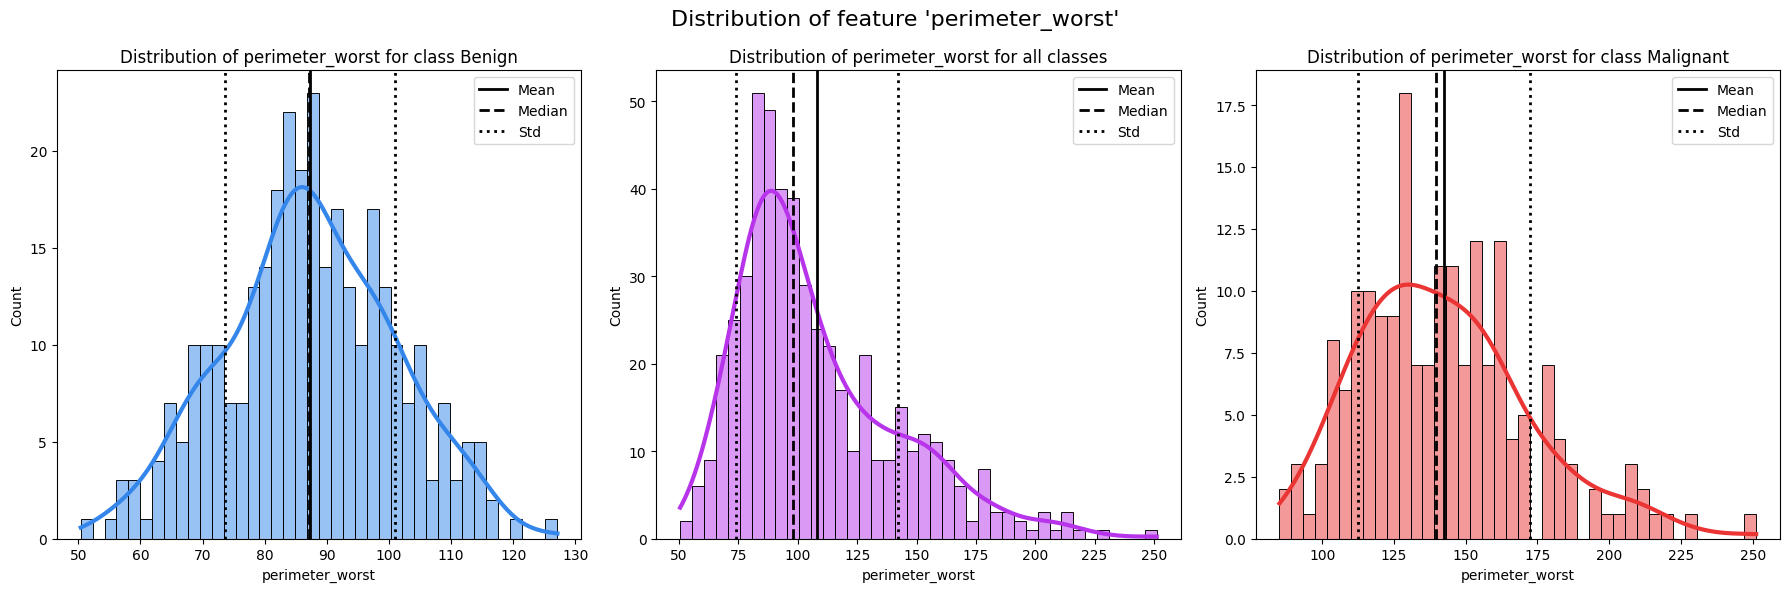
\includegraphics[width=\textwidth]{ims/perimeter_worst.png}
    \caption{Distribution of the \texttt{perimeter\_worst} feature for each
    class (left and right) and the whole dataset (center).}
    \label{fig:perimeter_worst}
\end{figure}

\begin{figure}[H]
    \centering
    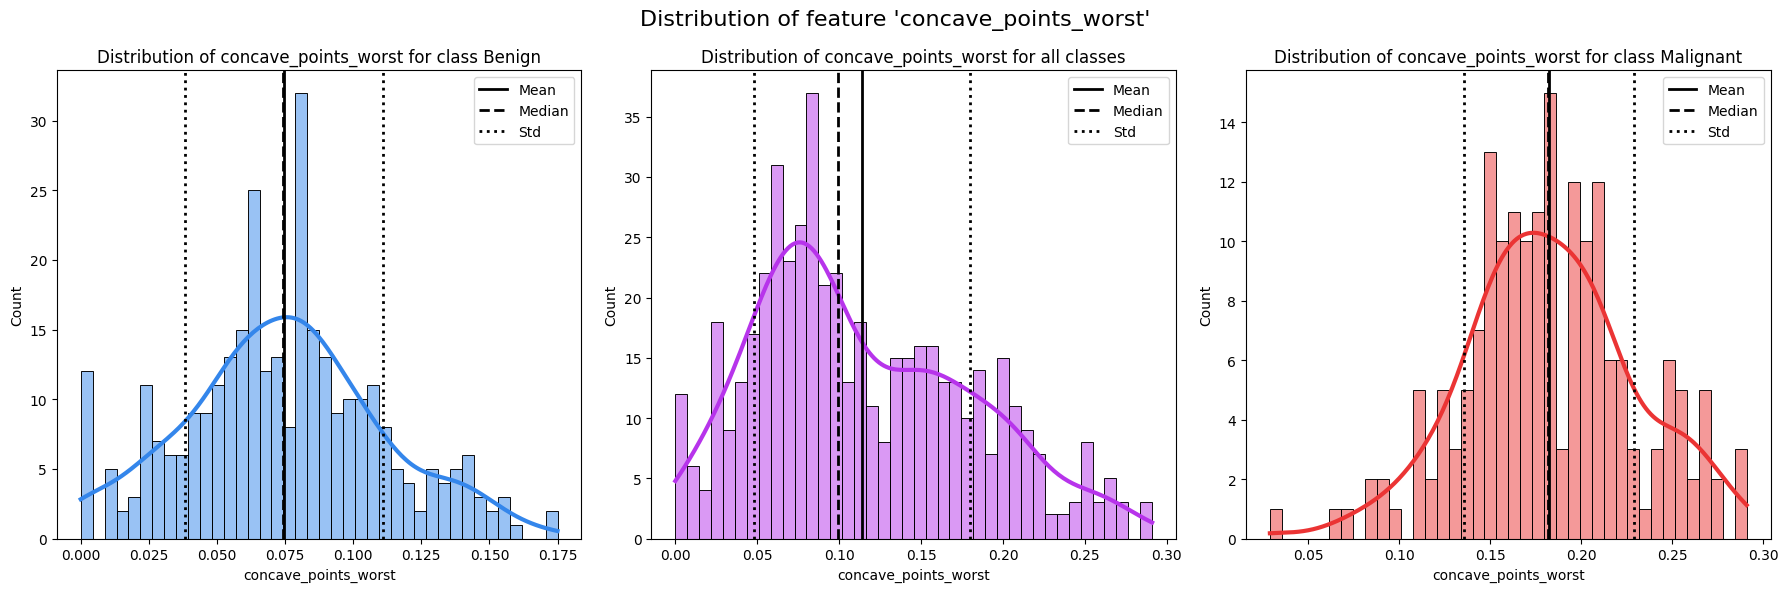
\includegraphics[width=\textwidth]{ims/concave_points_worst.png}
    \caption{Distribution of the \texttt{concave\_point\_worst} feature for each
    class (left and right) and the whole dataset (center).}
    \label{fig:area_worst}
\end{figure}

\begin{figure}[H]
    \centering
    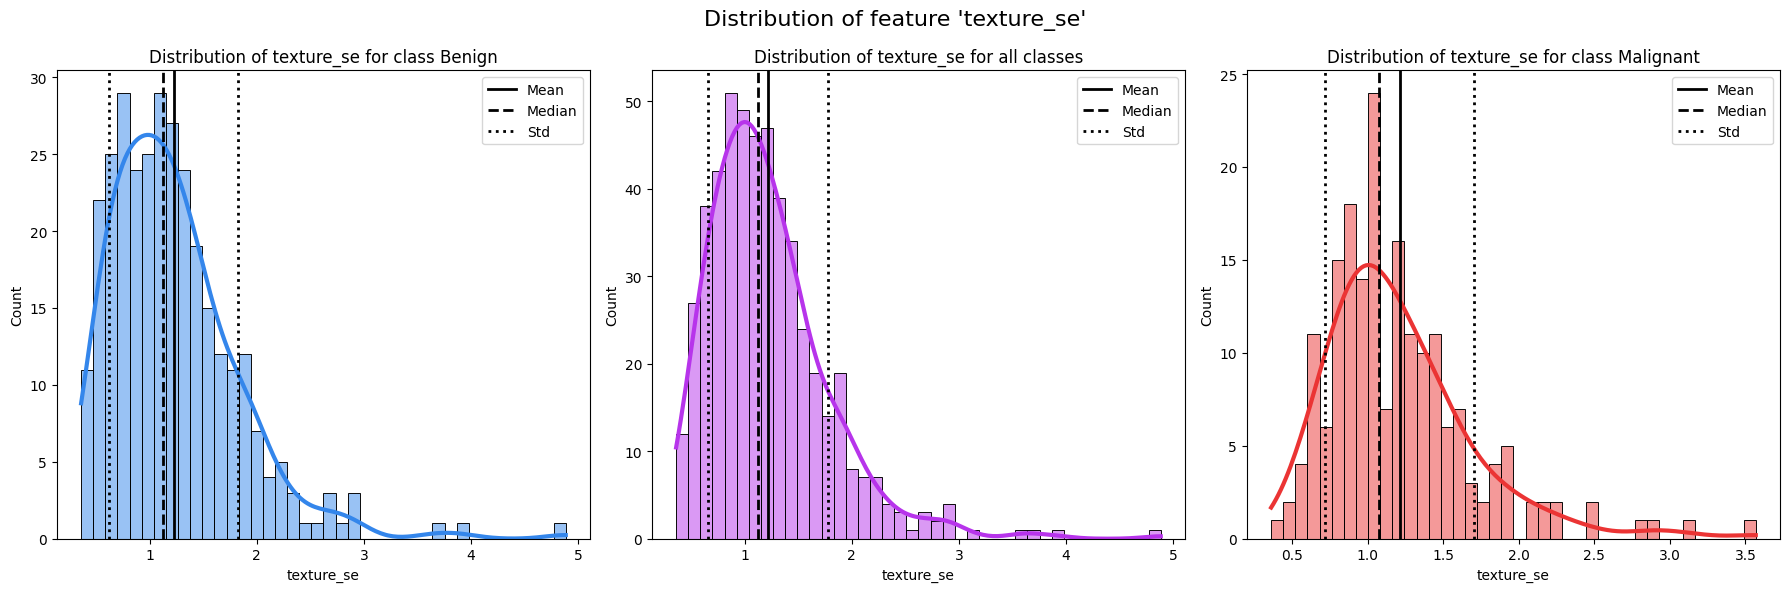
\includegraphics[width=\textwidth]{ims/texture_se.png}
    \caption{Distribution of the \texttt{texture\_se} feature for each class
    (left and right) and the whole dataset (center).}
    \label{fig:concave_points_se}
\end{figure}

In Figure~\ref{fig:perimeter_worst} and Figure~\ref{fig:area_worst}, we can see
that the two classes are well separated, with the malignant class having higher
values for both features. This is not the case in Figure~\ref{%
fig:concave_points_se}; the \texttt{concave\_points\_se} feature has very
similar distributions for both classes.

Next, we can inspect how correlated the features are with the target values by
calculating and plotting the Spearman's $\rho$, Kendall's $\tau$ and the Point
Biserial correlation coefficients. Spearman's $\rho$ and Kendalls's $\tau$ are
useful for measuring non-linear, monotonically increasing relations and the
Point Biserial correlation is specifically designed for binary classification
problems.

In Figure~\ref{fig:corr_coeffs} we can see the absolute values of the
correlation coefficients mentioned above. Eleven values show an absolute
correlation of above 0.6, while only seven being below 0.3, indicating that
the dataset has features that can describe the target value with high accuracy.

\begin{figure}[H]
    \centering
    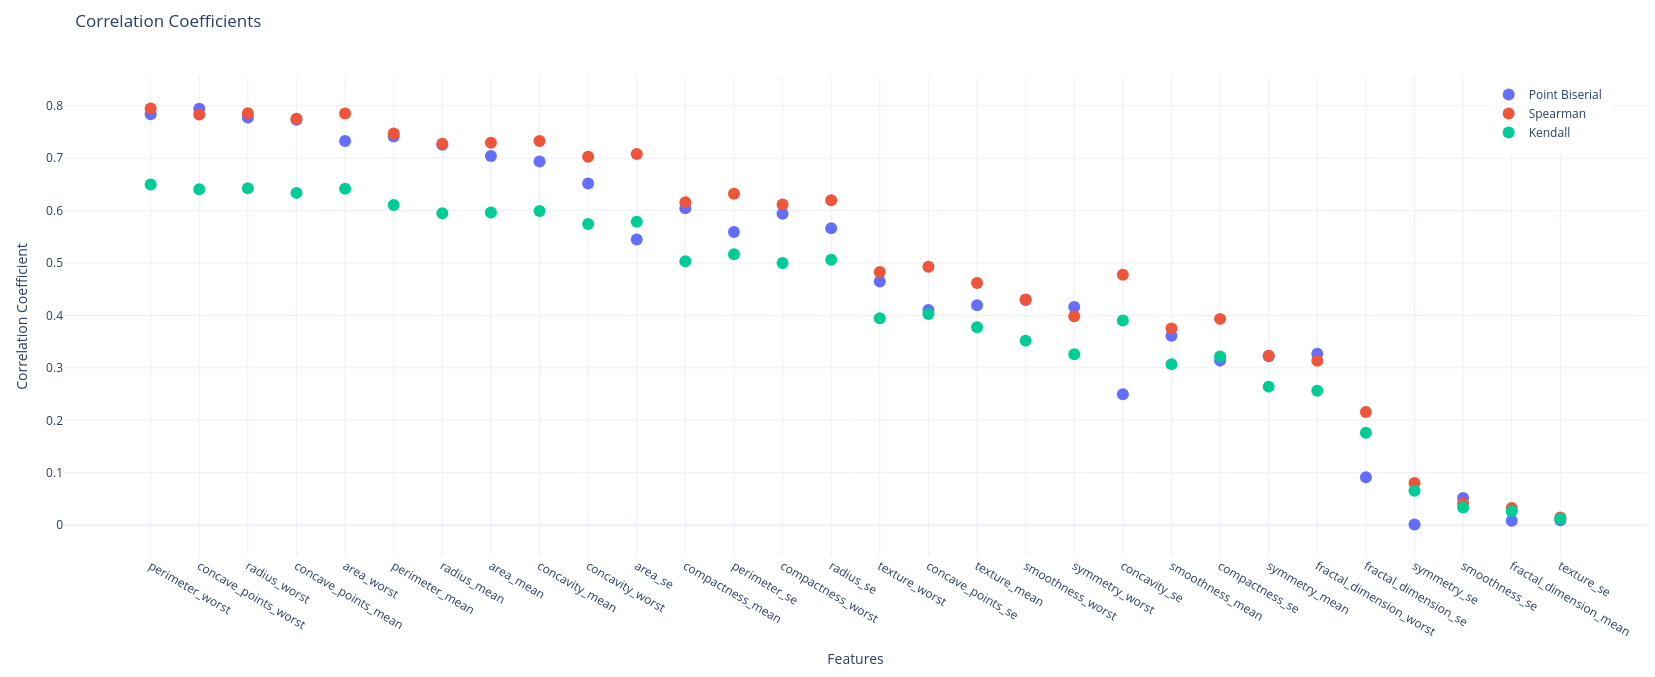
\includegraphics[width=\textwidth]{ims/corr_coeffs.png}
    \caption{Distribution of the Spearman's $\rho$ (red), Kendall's $\tau$
    (green), and Point Biserial (blue) correlation coefficients of all features
    with the target value.}
    \label{fig:corr_coeffs}
\end{figure}

Measuring and plotting the inter-feature correlation can help us find redundant
features. In Figure\ref{fig:corr_coeffs_heatmap} we can see a few examples of
features that seem to carry the same information; these groups of features
appear as spots of high correlation. For example the set of features regarding
the perimeter and radius show high intra-feature correlation, as well as high
correlation with the features regarding the area. Since I have ordered the
features alphabetically, we expect correlations along the main diagonal to
have high correlation, as they describe the correlation of features that
describe the same property, and we see that in four main ``blocks''.

\begin{figure}[H]
    \centering
    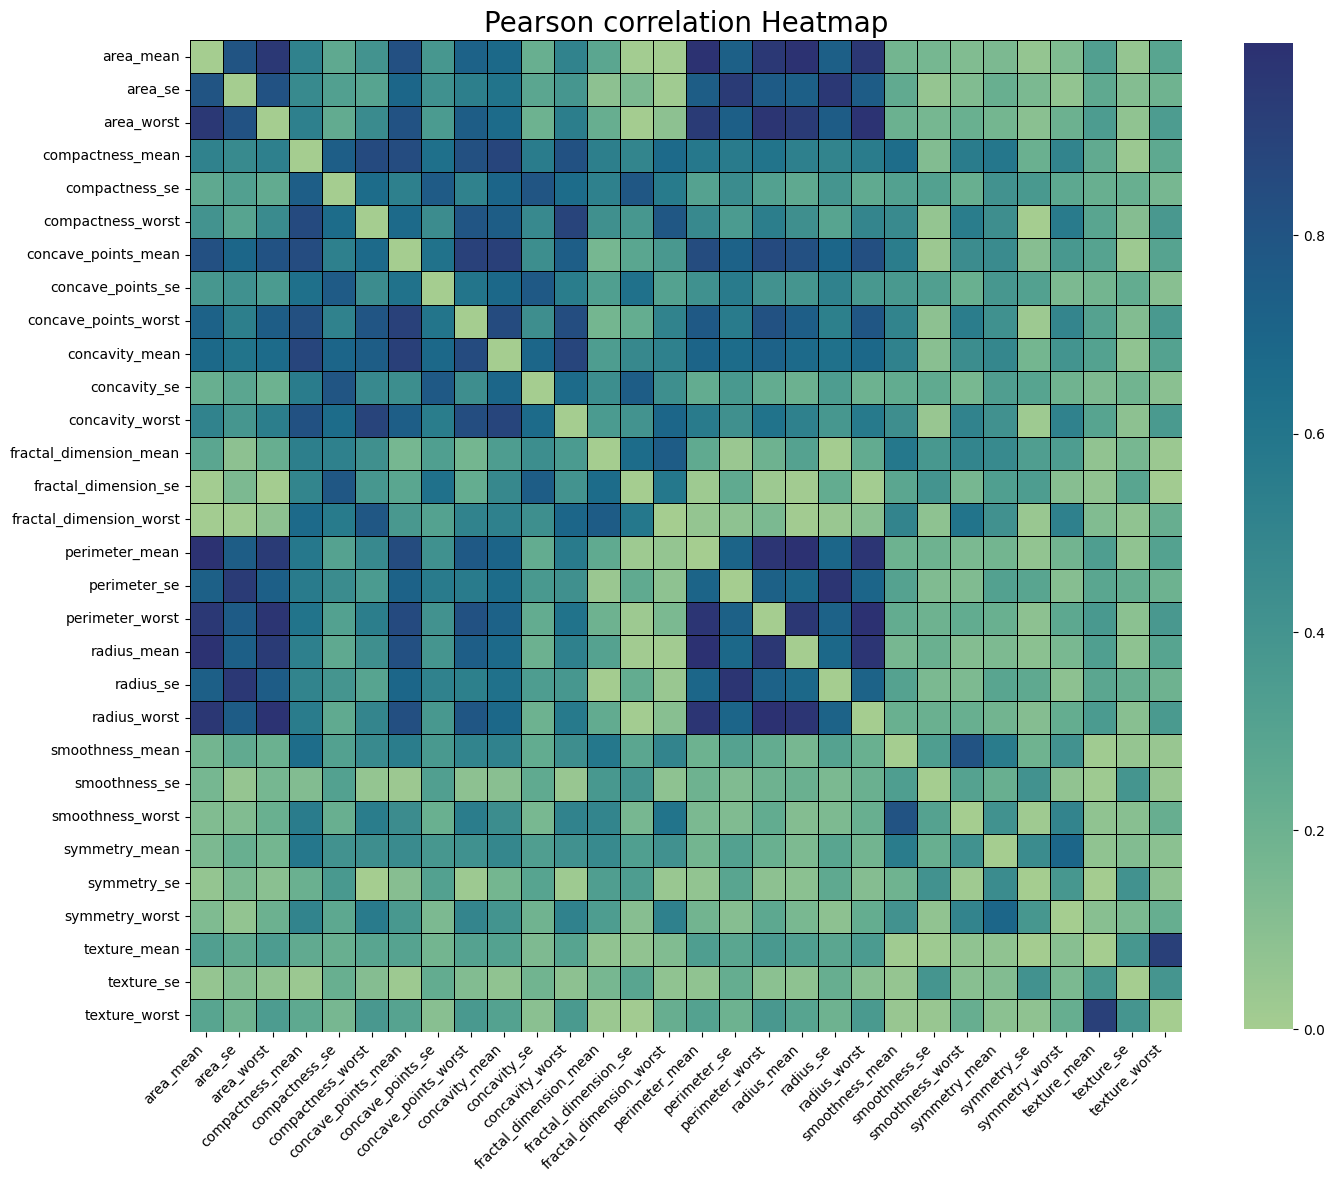
\includegraphics[width=\textwidth]{ims/corr_coeffs_heatmap.png}
    \caption{Distribution of the Spearman's $\rho$ (red), Kendall's $\tau$
    (green), and Point Biserial (blue) correlation coefficients of all features
    with the target value.}
    \label{fig:corr_coeffs_heatmap}
\end{figure}

Overall, the dataset seems to be well separated, with some features being
redundant. I expect that the classifiers will perform well, but I will need to
use feature selection to remove the redundant features and improve the
performance of the classifiers.

Latsly, we can use a dimensionality reduction technique to inspect if the
projections of the data to a subspace show any meaningful separation or if they
form any discernible structure. To that end I used \texttt{PCA}, \texttt{t-SNE},
and \texttt{UMAP} to map the data points onto a lower dimension and visualize
them. Below, I provide the plots for \texttt{PCA} and \texttt{UMAP}, the
\texttt{t-SNE} results are very similar to the results from \texttt{UAMP} and
they can be found in the \texttt{data\_exploration.ipynb} notebook, I will not
include them here for brevity.

In Figure~\ref{fig:pca} we can see that for the combination of the first and
second principal components, the data set can be somewhat separated, with the
benign class forming a more compact group and the malignant class forming a more
diffuse group, but there is no physical separation between them. A similar
case is true for the combination of the rest of the components. On the other
hand, in Figure~\ref{fig:umap}, we can see that the data points are separated
more clearly, forming a single elongated cluster of points which can be
separated almost exactly at its center, separating the two classes (in the
cases of the combinations of first and second dimension and first and third).
Furthermore, even in the first dimension, the data seem to from a binomial
distribution, separating the two classes.

\begin{figure}[H]
    \centering
    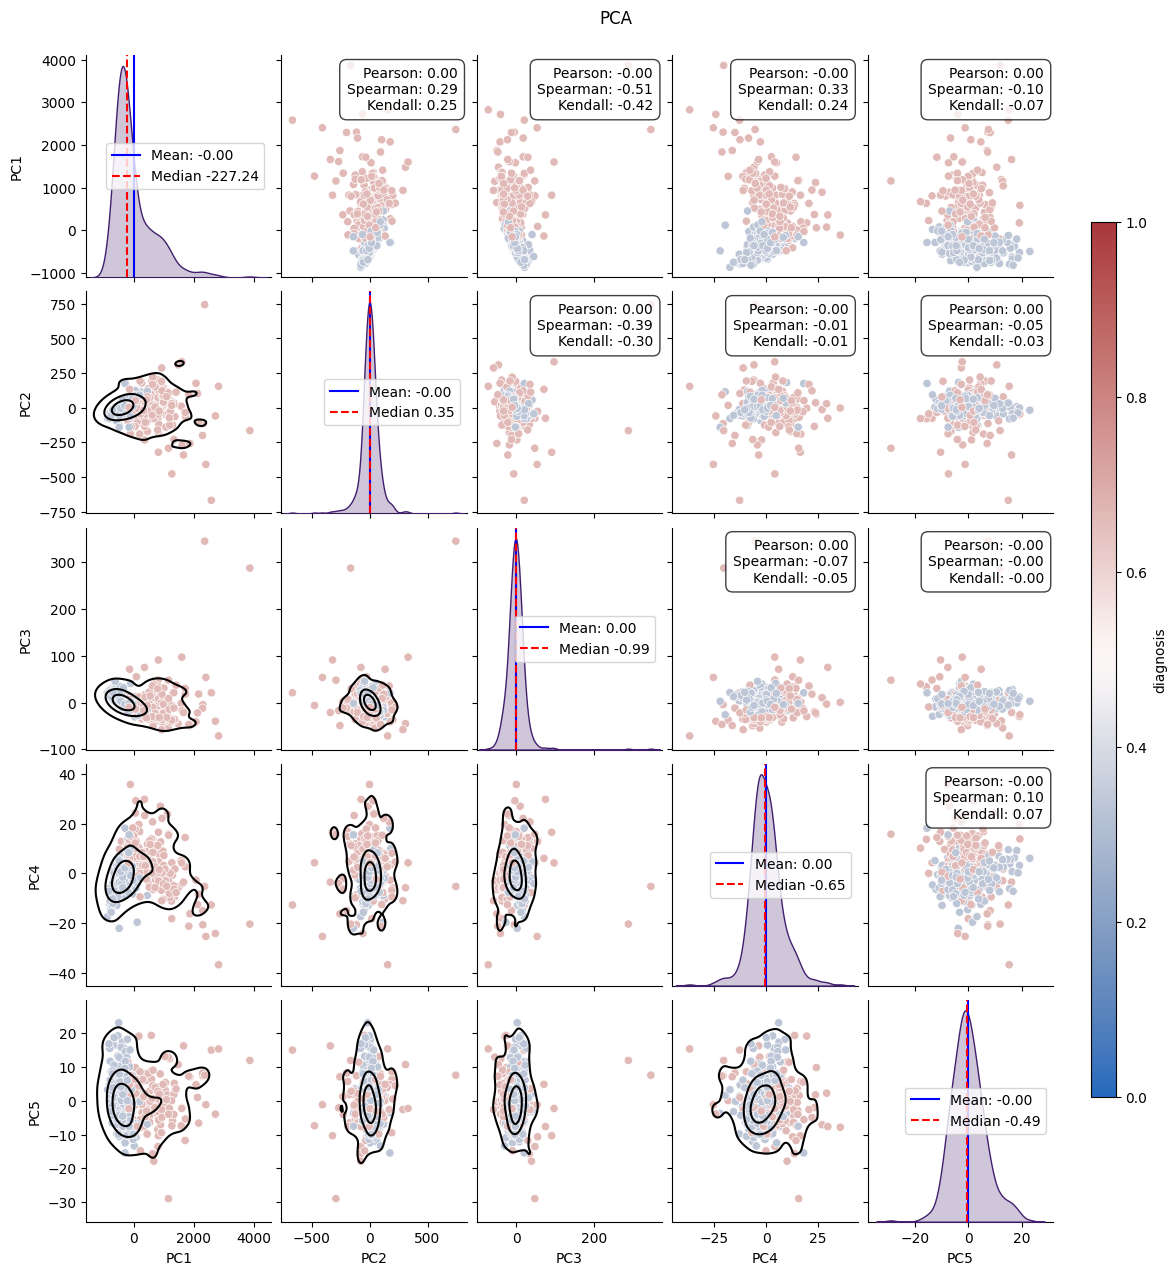
\includegraphics[width=\textwidth]{ims/pca.png}
    \caption{Pairplot of the first 5 prinicpal components after dimensionality
    reduction with \texttt{PCA}. The scatter plots are colored by the target's
    label (blue for benign and red for malignant).}
    \label{fig:pca}
\end{figure}

\begin{figure}[H]
    \centering
    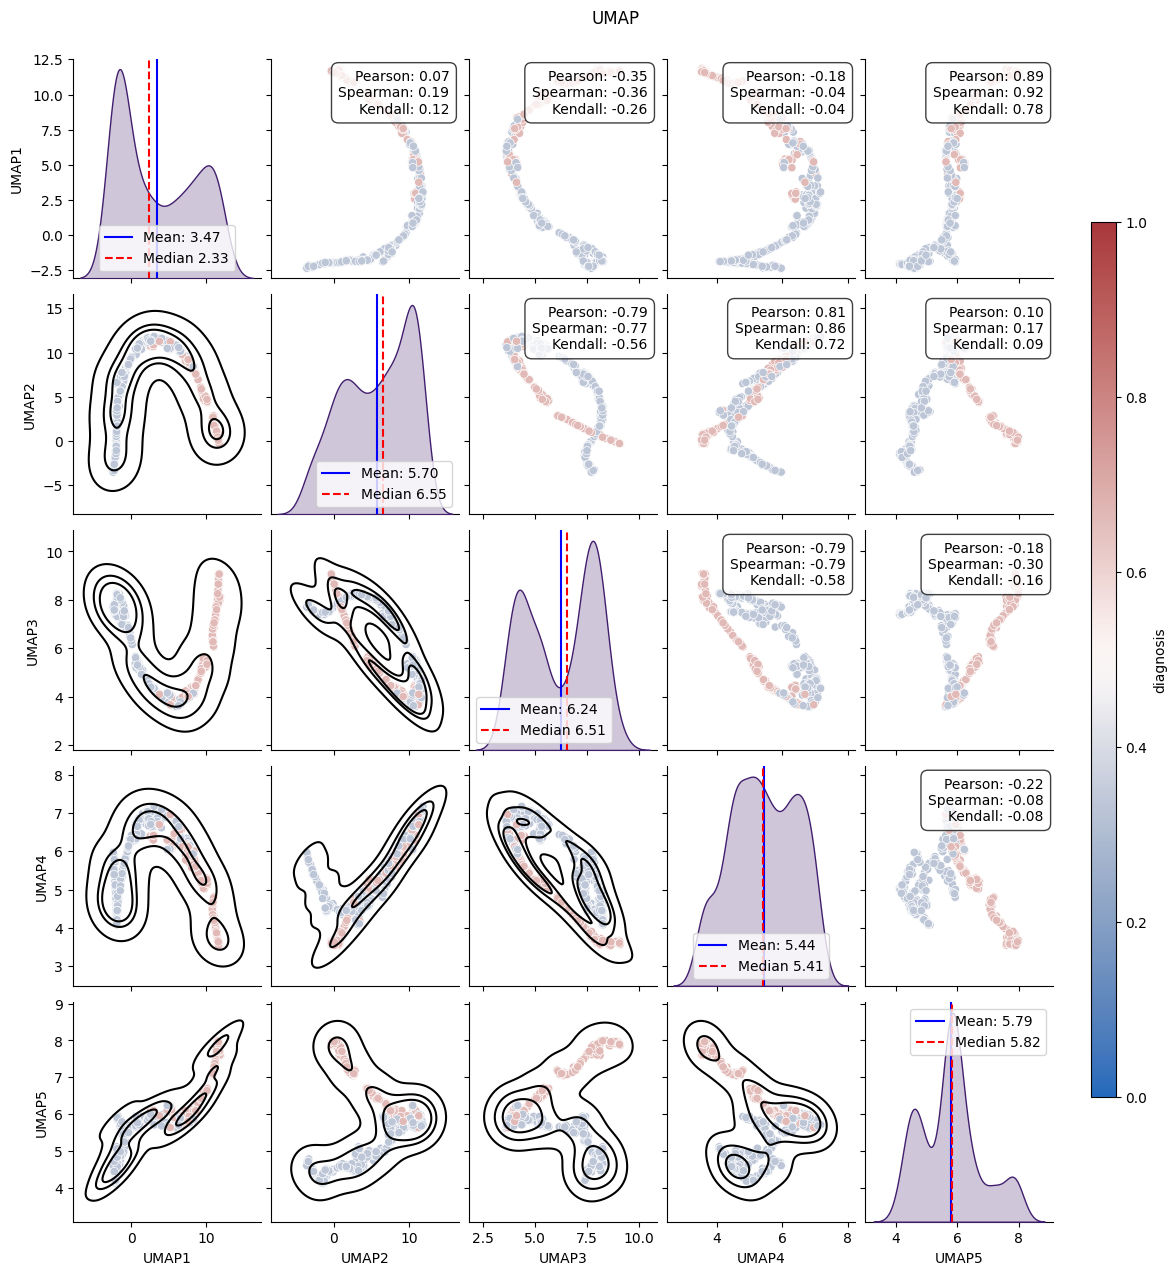
\includegraphics[width=\textwidth]{ims/umap.png}
    \caption{Pairplot of the first 5 embeddings / dimensions after
    dimensionality reduction with \texttt{UMAP}. The scatter plots are colored
    by the target's label (blue for benign and red for malignant).}
    \label{fig:umap}
\end{figure}

With all the above in mind, I decided to set up the \texttt{mRMR} function to
select 10 features, as I have shown that there are 11 features that have a
high correlation with the target value. Also I believe that the number is not
too high, so that the classifiers will be able to learn the underlying
patterns in relatively few iterations, but not too low so that the classifiers
will not be able to learn the underlying patterns.

%%%%%%%%%%%%%%%%%%%%%%%%%%%%%%%%%%%%%%%%%%%%%%%%%%%%%%%%%%%%%%%%%%%%%%%%%%%%%%%%
%%%%%%%%%%%%%%%%%%%%%%%%%%%%%%%%%%%%%%%%%%%%%%%%%%%%%%%%%%%%%%%%%%%%%%%%%%%%%%%%
\section{Material and methods}

%%%%%%%%%%%%%%%%%%%%%%%%%%%%%%%%%%%%%%%%%%%%%%%%%%%%%%%%%%%%%%%%%%%%%%%%%%%%%%%%
\subsection{Outline}

In essence, a nested cross-validation pipeline consists of two nested loops
(outer and inner loops), encapsulated in a larger loop. In our case, the
encapsulating loops (or rounds) will be set to $R=10$, the outer loops will be
set to $N=5$, and the inner loops to $K=3$.

The job of the outer fold is to split the data set and perform cross-validation,
with the inner folds performing hyperparameter tuning with yet another
cross-validation. The job of the enclosing rounds is to change the random number
generator seeds, to get $R$ different results, leading to better generalization
ability of the model. A schematic of nested cross-validation is provided below
(Figure\ref{fig:ncv_scheme}).

\begin{figure}[H]
    \centering
    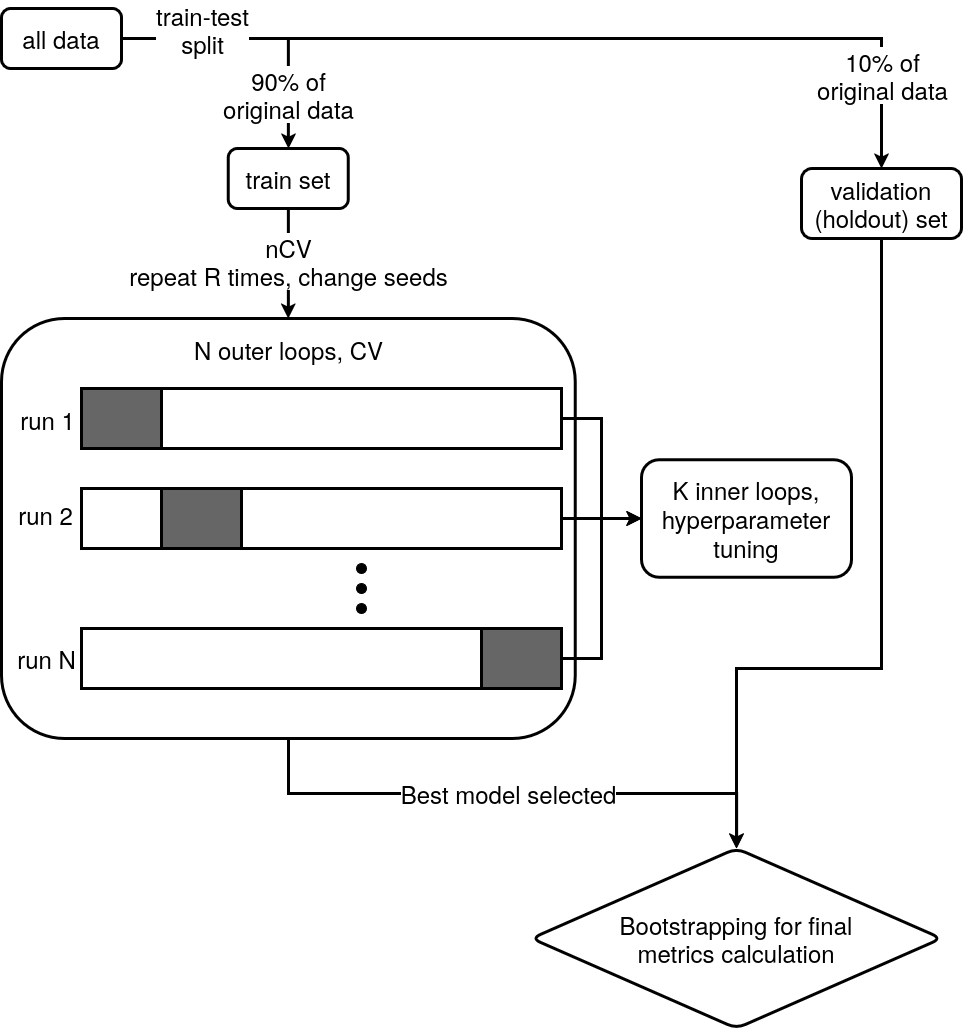
\includegraphics[width=0.75\textwidth]{ims/nCV.drawio.png}
    \caption{Nested cross-validation scheme. A holdout set is first taken from
    the dataset, here set to $10\%$. Then, $R$ times, the model is trained
    using cross-validation ($N$ splits), with an inner loop of hyperparameter
    tuning, which is also done using cross-validation ($K$ splits). All
    training results are aggregated and the best set of hyperparameters
    is selected. After all models are trained, the best one can be tested
    against the unseen data (holdout set); here metric statistics are
    calculated using resampling with bootstrapping.}
    \label{fig:ncv_scheme}
\end{figure}

The implementation of a nested cross-validation is easy, but it needs extra
care to avoid data leakage. The data must be scaled inside the inner loop, after
their final split, otherwise the training set will carry some information of the
test set (and as always the scaler must be fitted only on the test
set)~\cite{Bates_2023}. I decided to perform feature selection using the whole
training set, ignoring the fact that it might ``leak'' some information to the
rest of the pipeline, as I believe it will be minimal and doing otherwise would
have been ``overkill'' in this case.


%%%%%%%%%%%%%%%%%%%%%%%%%%%%%%%%%%%%%%%%%%%%%%%%%%%%%%%%%%%%%%%%%%%%%%%%%%%%%%%%
\subsection{Feature selection}

As part of the bonus questions, I also performed feature selection with two
methods. The first was using the \texttt{mRMR}~\cite{mRMR} method which aims to
minimize the redundancy between features and maximize their relevance to the
target value; to that end, I used the \texttt{pymrmr}\footnote{\url{%
https://github.com/fbrundu/pymrmr}} package.

The second was more unorthodox. Since seeing the embeddings produced by
\texttt{UMAP} and how well the classes were separated in that subspace, I
decided to transform the dataset using \texttt{UMAP} and generate new features.
The disadvantage here is that the results will no longer be interpretable and
the mapper will have to also be saved and incorporated in the pipeline for
the model to be able to classify unseen data.


%%%%%%%%%%%%%%%%%%%%%%%%%%%%%%%%%%%%%%%%%%%%%%%%%%%%%%%%%%%%%%%%%%%%%%%%%%%%%%%%
\subsection{Hyperparameter tuning}

Hyperparameter tuning was performed inside the inner loop of the nested
cross-validation. The hyperparameters were tuned using the \texttt{optimize}
method of the \texttt{Optuna}\footnote{%
\url{https://optuna.org/}} library with a \texttt{TPE} sampler, which fits
one Gaussian mixture model ($l(x)$) to the set of parameters associated with the
best objective values and another ($g(x)$) to the remaining parameters and tries
to maximize the ratio of the two, ($\frac{l(x)}{g(x)}$). The objective function
uses the Matthews correlation coefficient (MCC)~\cite{Chicco2023} as the metric
to evaluate the performance of the model.


%%%%%%%%%%%%%%%%%%%%%%%%%%%%%%%%%%%%%%%%%%%%%%%%%%%%%%%%%%%%%%%%%%%%%%%%%%%%%%%%
\subsection{Model selection --- best model final training}

After the nested cross-validation is complete, the best model is selected
manually based on the over-all statistics. The selected model is fit on the
complete dataset (minus the holdout set) using the features and hyperparameters
selected and finally it is tested against the holdout set with 1000 rounds of
resampling with bootstrapping to generate enough samples to calculate
statistics.


%%%%%%%%%%%%%%%%%%%%%%%%%%%%%%%%%%%%%%%%%%%%%%%%%%%%%%%%%%%%%%%%%%%%%%%%%%%%%%%%
%%%%%%%%%%%%%%%%%%%%%%%%%%%%%%%%%%%%%%%%%%%%%%%%%%%%%%%%%%%%%%%%%%%%%%%%%%%%%%%%
\section{Results and discussion}

The complete process for $R=10$, $N=5$, and $K=3$, and for 100 \texttt{Optuna}
trials, for all classifiers, took around one hour, on a machine running Ubuntu
24, with 16 GB of RAM, an AMD Ryzen 7 5800H processor, and an NVIDIA GeForce RTX
3050 Ti graphics card. All classifiers trained at relatively similar speeds,
with the exception of RF and LGBM, which took significantly more time than the
rest.

The complete training process can be viewed in the \texttt{classification.ipynb}
and in the \texttt{evaluation.ipynb} notebooks which containing the complete
training process and the visualization of all results.


%%%%%%%%%%%%%%%%%%%%%%%%%%%%%%%%%%%%%%%%%%%%%%%%%%%%%%%%%%%%%%%%%%%%%%%%%%%%%%%%
\subsection{Feature Selection}

Feature selection using \texttt{mRMR} or \texttt{UMAP} did not seem to improve
the performance of the tested classifiers. For reference we can see that the
baseline Logistic Regression model, which was also the best performing model,
has better metrics, with the median of all metrics being over 9.25!

\begin{figure}[H]
    \centering
    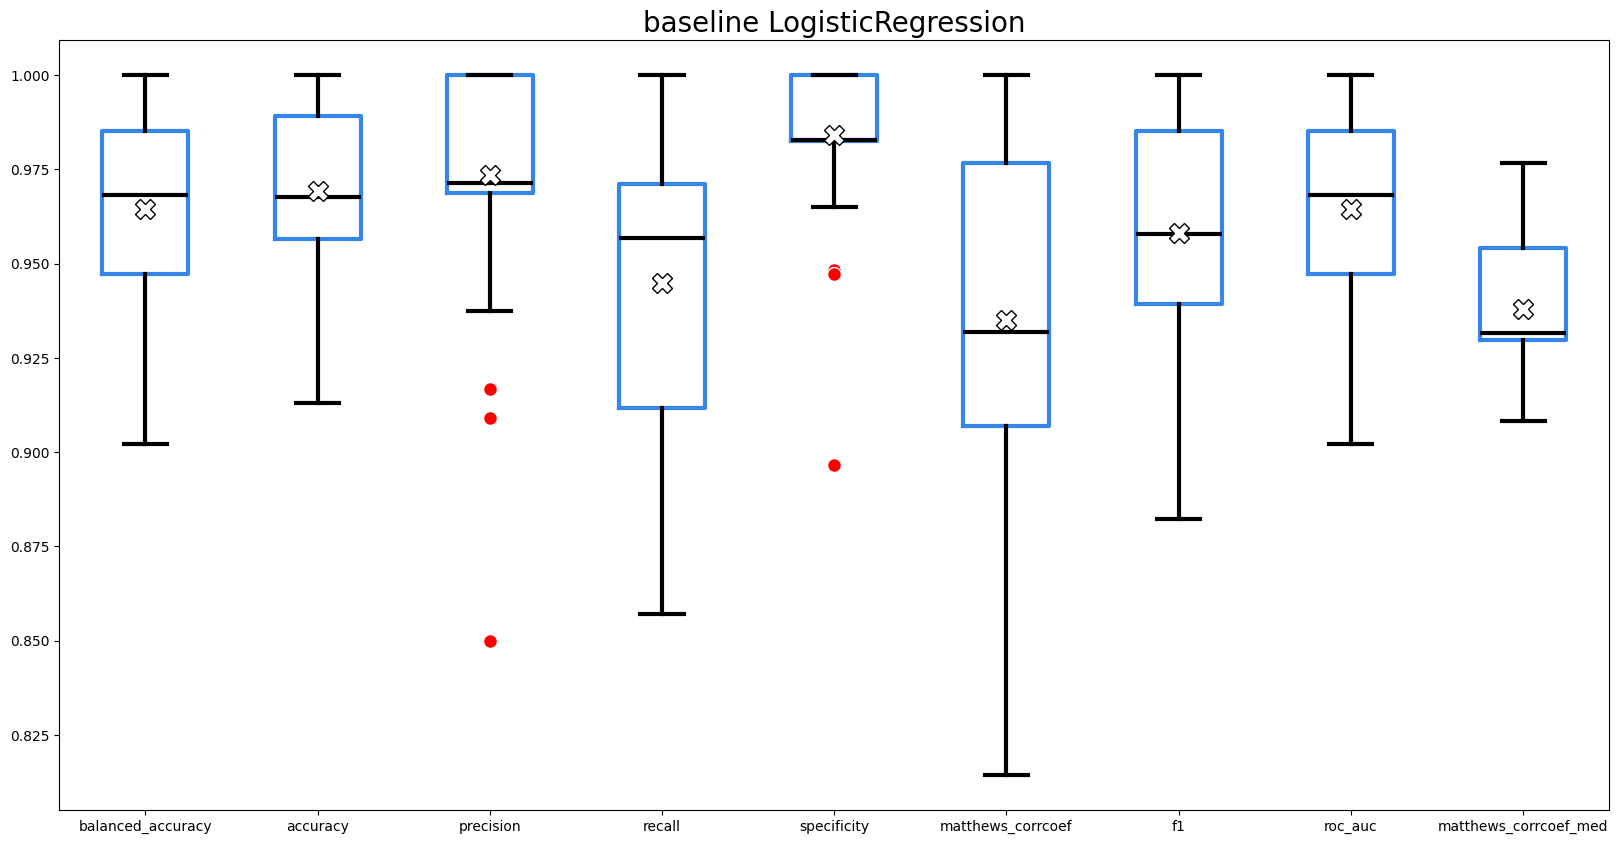
\includegraphics[width=\textwidth]{ims/baseline_logistic.png}
    \caption{Performance of the baseline LR model.}
    \label{fig:baseline_logistic}
\end{figure}

\begin{figure}[H]
    \centering
    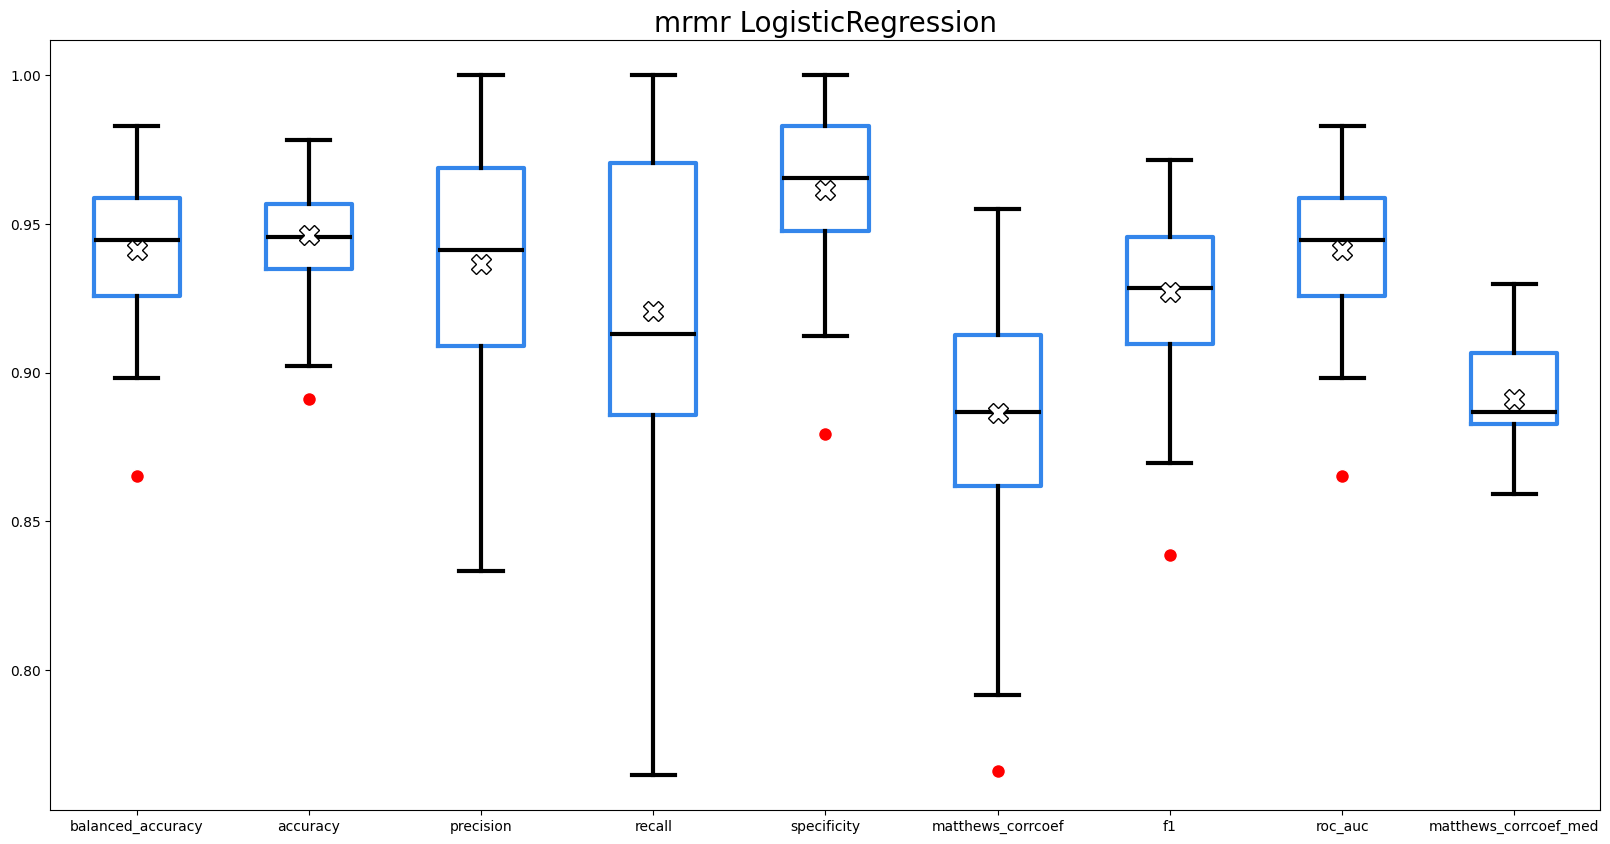
\includegraphics[width=\textwidth]{ims/mrmr_logistic.png}
    \caption{Performance of the baseline LR model with \texttt{mRMR}.}
    \label{fig:mrmr_logistic}
\end{figure}

\begin{figure}[H]
    \centering
    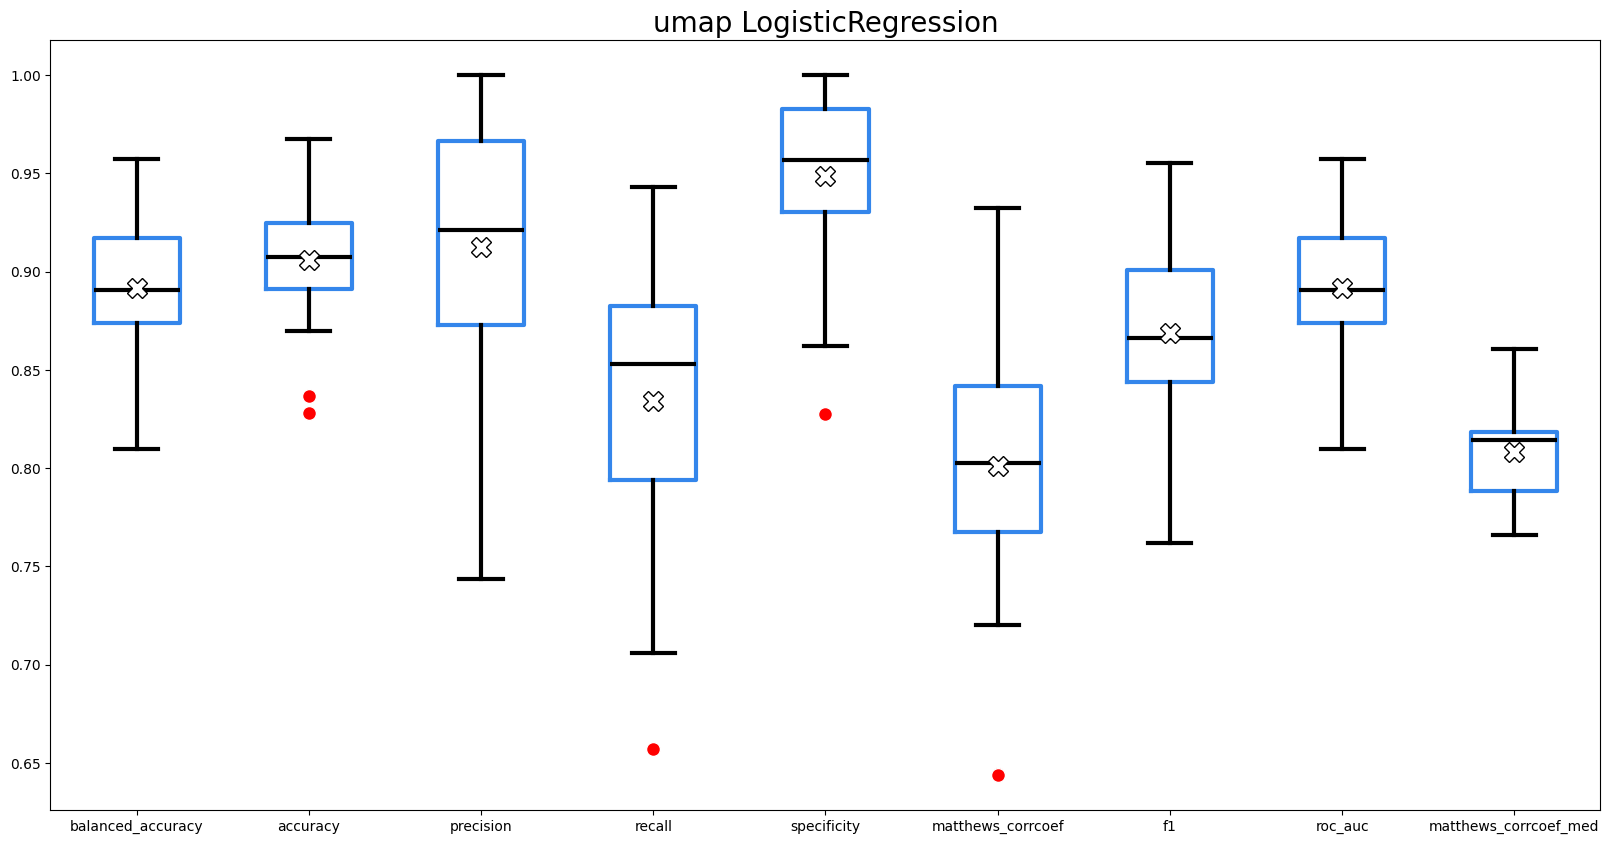
\includegraphics[width=\textwidth]{ims/umap_logistic.png}
    \caption{Performance of the baseline LR model with \texttt{UMAP}.}
    \label{fig:umap_logistic}
\end{figure}

%%%%%%%%%%%%%%%%%%%%%%%%%%%%%%%%%%%%%%%%%%%%%%%%%%%%%%%%%%%%%%%%%%%%%%%%%%%%%%%%
\subsection{Hyperparameters}

The hyperparameters chosen by \texttt{Optuna} during baseline training (no
feature selection) are provided in the Table below (Table~\ref{%
tab:hyperparams_models}).

\begin{table}[H]
    \centering
    \begin{tabular}{|c|c|c|}
    \hline
    \textbf{Model} & \textbf{Parameter} & \textbf{Value} \\
    \hline
    \multirow{4}{*}{LogisticRegression}
      & \texttt{C} & 43.7051 \\
      & \texttt{l1\_ratio} & 0.0536 \\
      & \texttt{max\_iter} & 1758 \\
      & \texttt{class\_weight} & None \\
    \hline
    \multirow{1}{*}{GaussianNB}
      & \texttt{var\_smoothing} & $1.94 \times 10^{-10}$ \\
    \hline
    \multirow{3}{*}{LinearDiscriminantAnalysis}
      & \texttt{solver} & lsqr \\
      & \texttt{shrinkage} & auto \\
      & \texttt{priors} & None \\
    \hline
    \multirow{5}{*}{SVC}
      & \texttt{C} & 0.8969 \\
      & \texttt{gamma} & auto \\
      & \texttt{coef0} & 0.0822 \\
      & \texttt{kernel} & linear \\
      & \texttt{class\_weight} & None \\
    \hline
    \multirow{3}{*}{RandomForestClassifier}
      & \texttt{n\_estimators} & 32 \\
      & \texttt{criterion} & gini \\
      & \texttt{min\_samples\_split} & 12 \\
    \hline
    \multirow{10}{*}{LGBMClassifier}
      & \texttt{boosting\_type} & dart \\
      & \texttt{num\_leaves} & 32 \\
      & \texttt{max\_depth} & 53 \\
      & \texttt{learning\_rate} & 0.4030 \\
      & \texttt{n\_estimators} & 903 \\
      & \texttt{min\_child\_samples} & 20 \\
      & \texttt{reg\_alpha} & 0.1486 \\
      & \texttt{reg\_lambda} & 0.5418 \\
      & \texttt{bagging\_freq} & 9 \\
      & \texttt{bagging\_fraction} & 0.4555 \\
      & \texttt{feature\_fraction} & 0.5883 \\
    \hline
    \end{tabular}
    \caption{Best hyperparameters for each classifier after tuning. Numerical
    values rounded for readability.}
    \label{tab:hyperparams_models}
\end{table}


%%%%%%%%%%%%%%%%%%%%%%%%%%%%%%%%%%%%%%%%%%%%%%%%%%%%%%%%%%%%%%%%%%%%%%%%%%%%%%%%
\subsection{Training results}

To capture the performance of the models the following metrics were used:
\begin{center}
    \texttt{balanced accuracy}
    $\bullet$
    \texttt{accuracy}
    $\bullet$
    \texttt{precision}
    $\bullet$
    \texttt{recall}
    $\bullet$
    \texttt{specificity}
    $\bullet$
    \texttt{MCC}
    $\bullet$
    \texttt{F1}
    $\bullet$
    \texttt{ROC AUC}
\end{center}

Below I include the boxplots for the MCC, recall, specificity, and balanced
accuracy metrics that the models achieved during their training (without
feature selection)
(Figures~\ref{fig:baseline_mcc},~\ref{fig:baseline_recall},~\ref{%
fig:baseline_specificity},~\ref{fig:baseline_balanced_accuracy}), the rest are
not included for brevity but they can be found in \texttt{evaluation.ipynb}.

From these metrics we can see that LR scored the best in all areas and even
achieved a median specificity of 1, without losing in recall, which is not
expected due to the recall/specificity tradeoff.
\[
recall = \frac{TP}{TP + FN}
\]
\[
specificity = \frac{TN}{TN + FP}
\]


\begin{figure}[H]
    \centering
    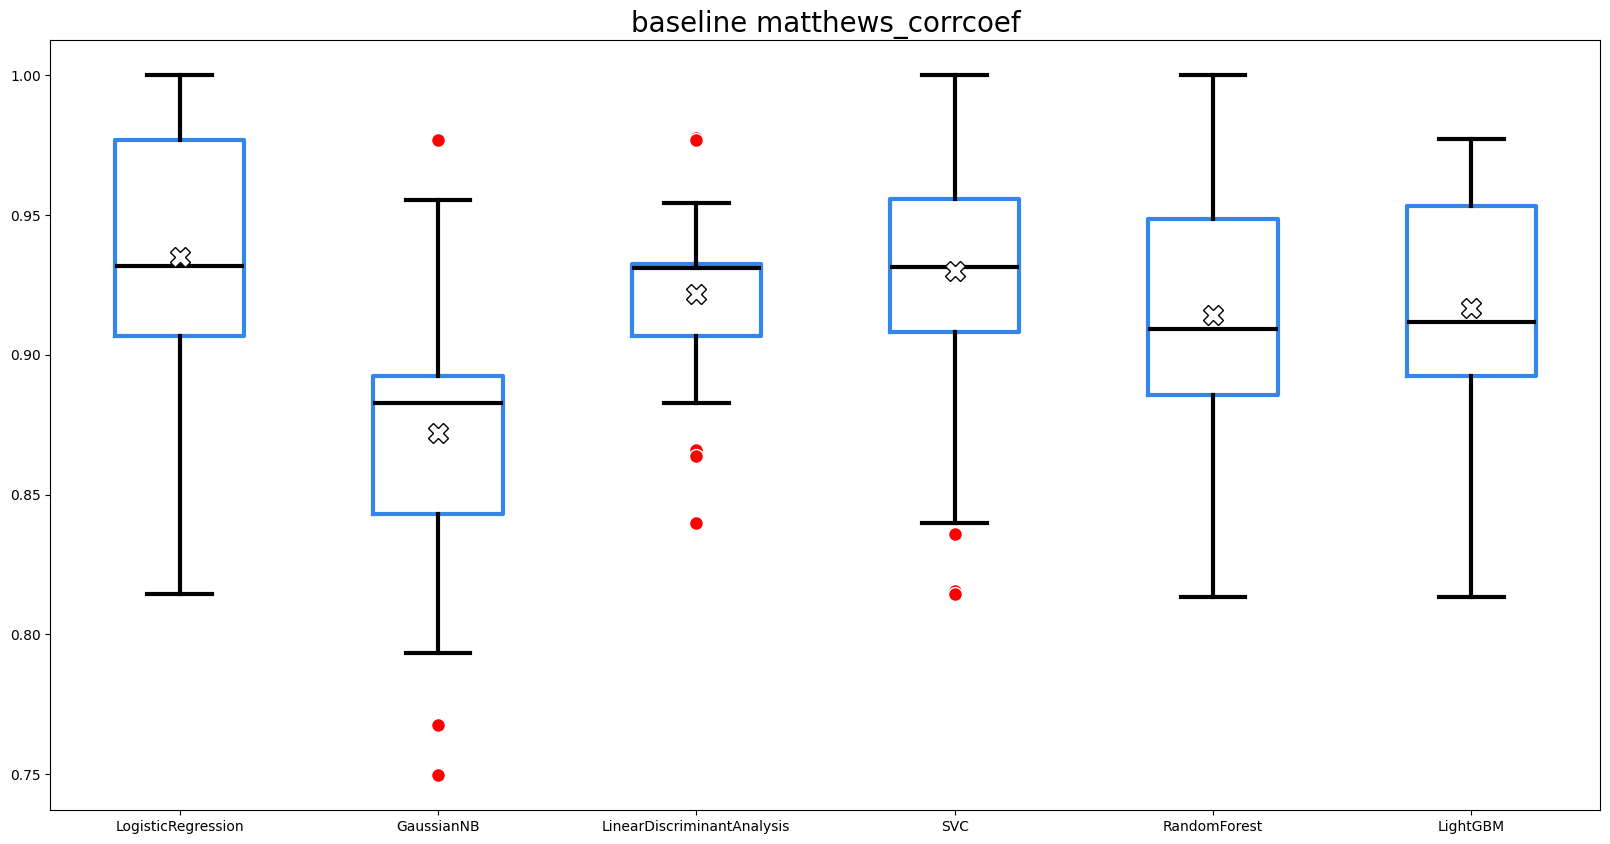
\includegraphics[width=\textwidth]{ims/baseline_mcc.png}
    \caption{Matthews correlation coefficient for all models.}
    \label{fig:baseline_mcc}
\end{figure}

\begin{figure}[H]
    \centering
    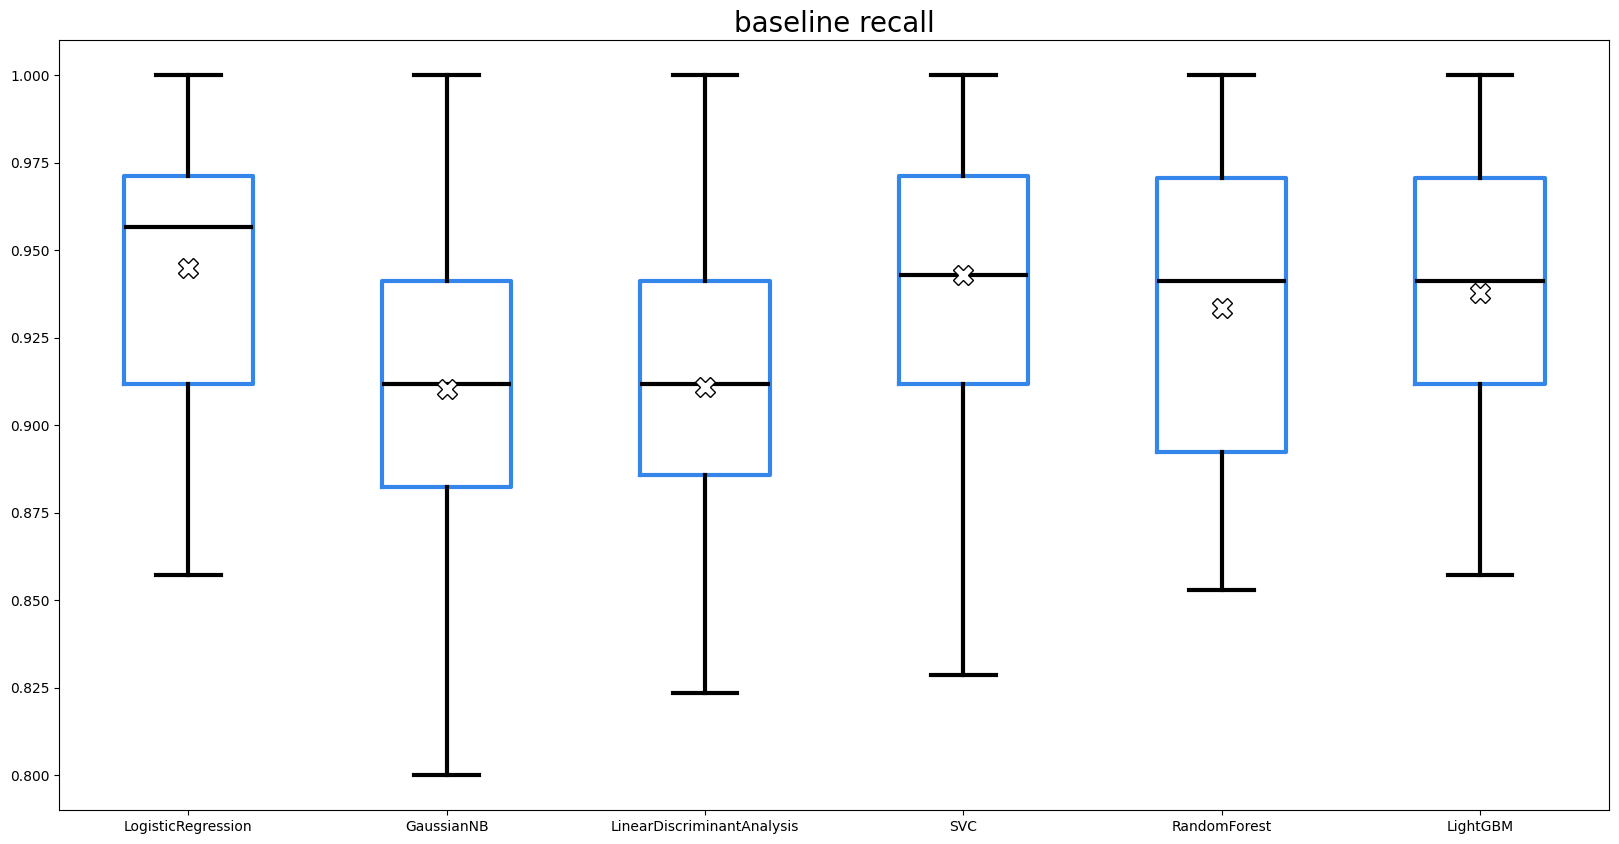
\includegraphics[width=\textwidth]{ims/baseline_recall.png}
    \caption{Recall for all models.}
    \label{fig:baseline_recall}
\end{figure}

\begin{figure}[H]
    \centering
    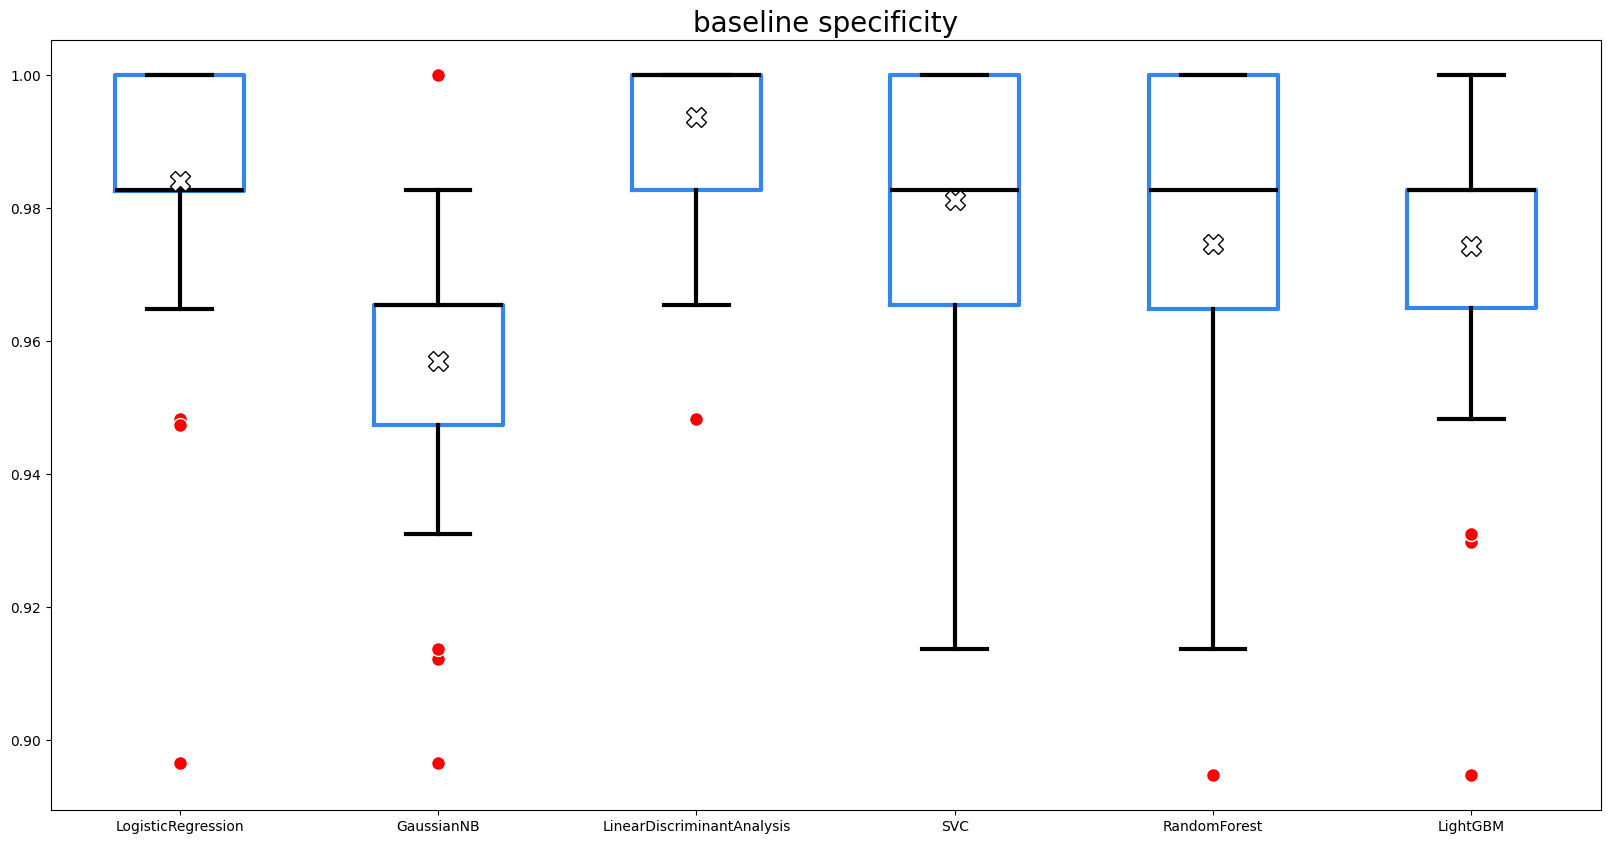
\includegraphics[width=\textwidth]{ims/baseline_specificity.png}
    \caption{Specificity for all models.}
    \label{fig:baseline_specificity}
\end{figure}

\begin{figure}[H]
    \centering
    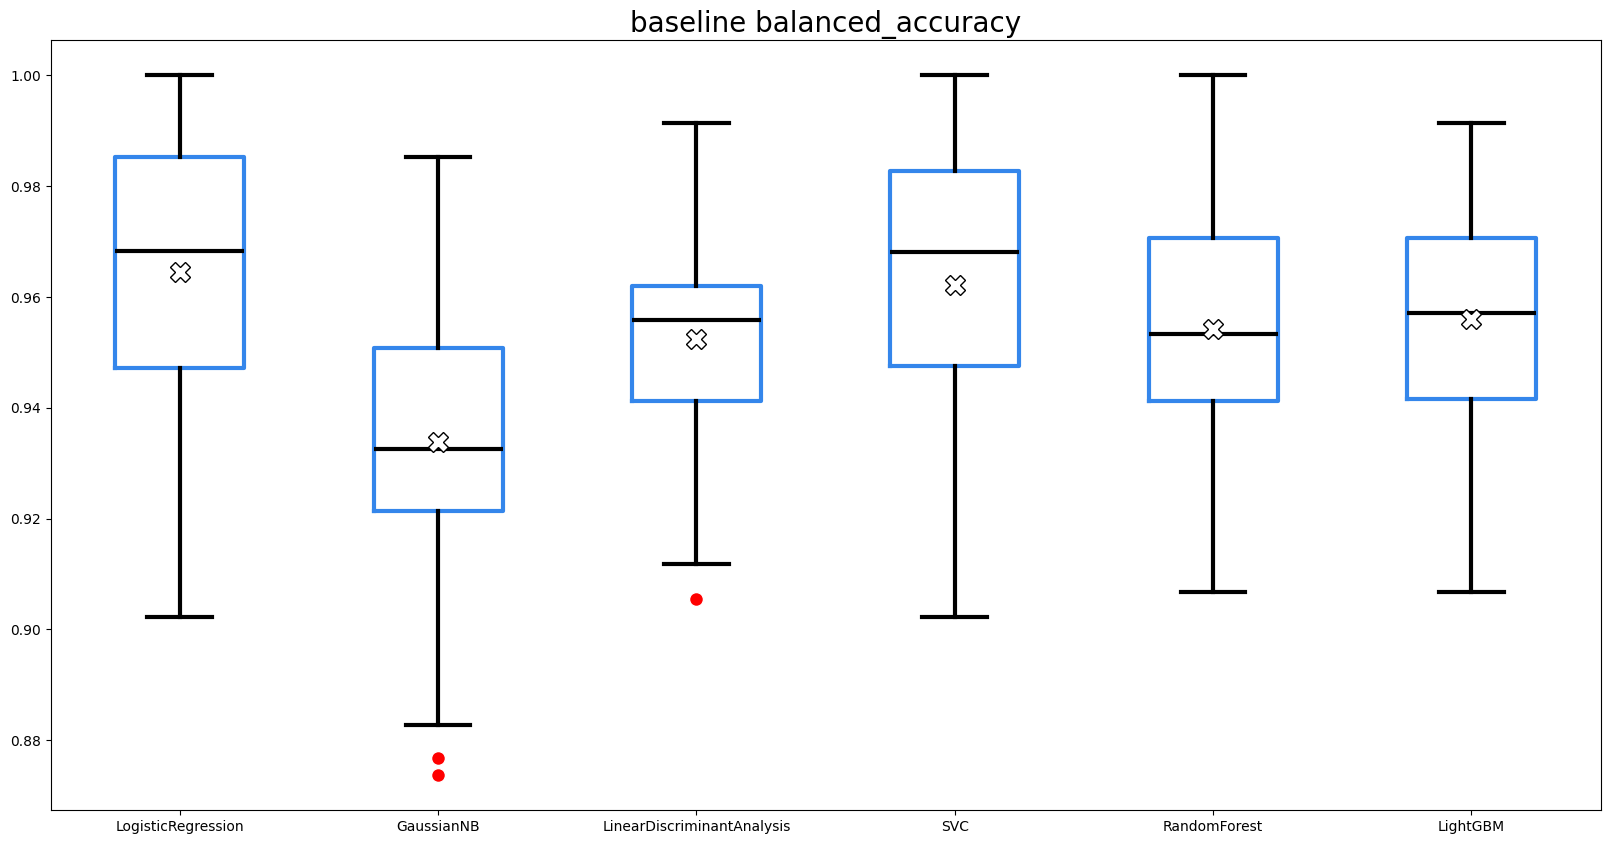
\includegraphics[width=\textwidth]{ims/baseline_balanced_accuracy.png}
    \caption{Balanced accuracy for all models.}
    \label{fig:baseline_balanced_accuracy}
\end{figure}


%%%%%%%%%%%%%%%%%%%%%%%%%%%%%%%%%%%%%%%%%%%%%%%%%%%%%%%%%%%%%%%%%%%%%%%%%%%%%%%%
\subsection{Best model evaluation}

The best model was then tested against the holdout set, using the same metrics
as above and 1000 rounds of resampling with bootstrapping to generate enough
samples to calculate statistics. The results are shown in Figure~\ref{%
fig:best_model_eval}.

\begin{figure}[H]
    \centering
    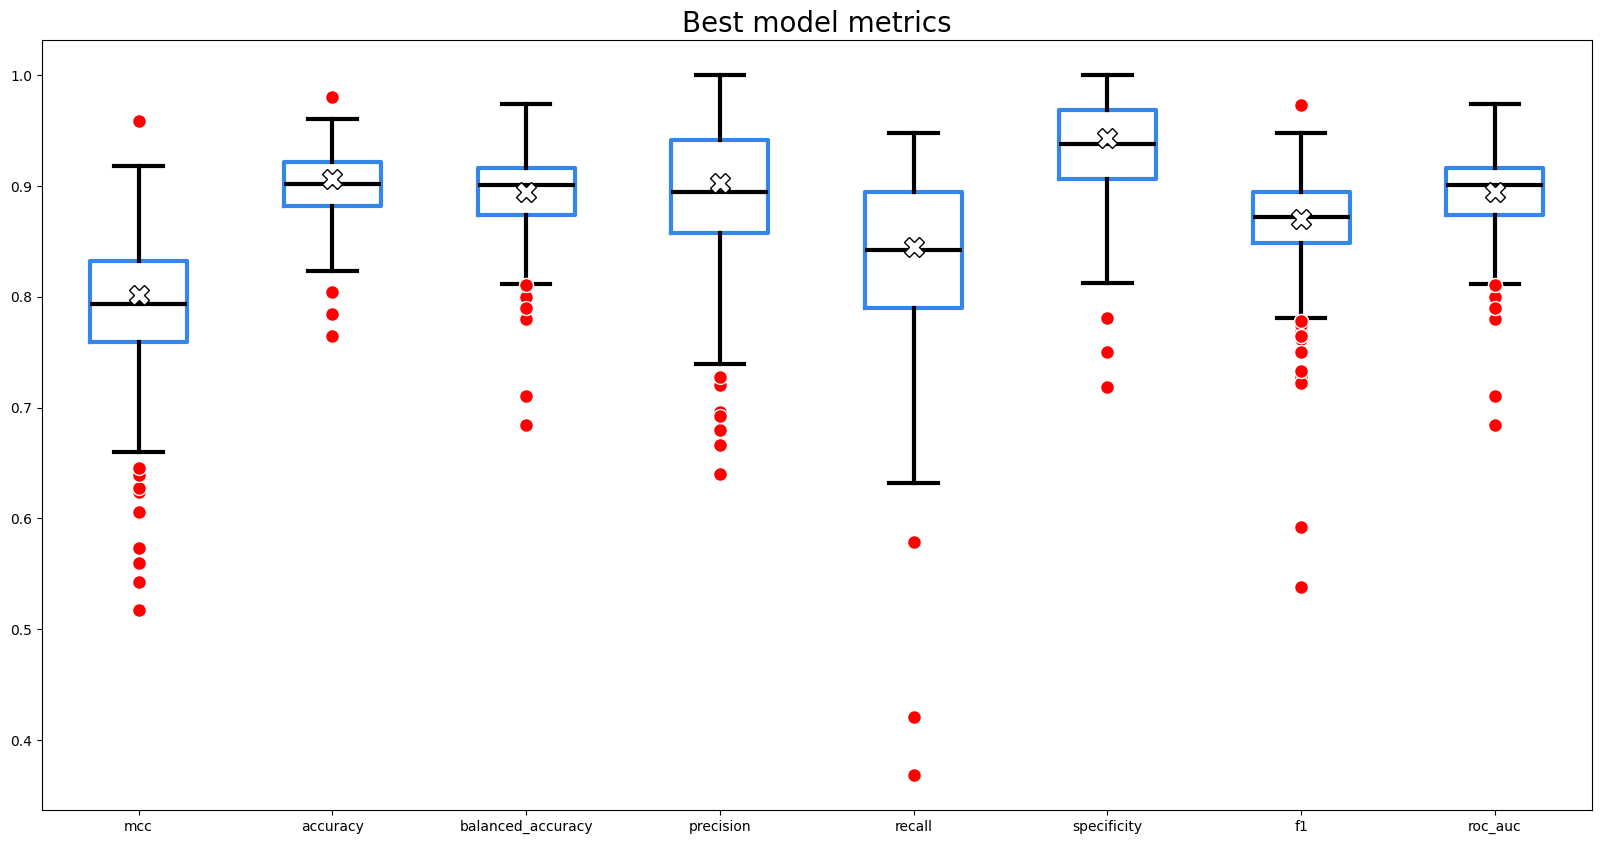
\includegraphics[width=\textwidth]{ims/best.png}
    \caption{Best model evaluation metrics.}
    \label{fig:best_model_eval}
\end{figure}



%%%%%%%%%%%%%%%%%%%%%%%%%%%%%%%%%%%%%%%%%%%%%%%%%%%%%%%%%%%%%%%%%%%%%%%%%%%%%%%%
%%%%%%%%%%%%%%%%%%%%%%%%%%%%%%%%%%%%%%%%%%%%%%%%%%%%%%%%%%%%%%%%%%%%%%%%%%%%%%%%
\section{Conclusion}

Nested cross-validation is a robust approach for training machine learning
models, particularly when paired with advanced feature selection and
hyperparameter optimization techniques such as \texttt{mRMR} and
\texttt{Optuna}. A Linear Discriminant Analysis model achieved excellent
performance on unseen data, with precision and specificity of 1.0, accuracy, F1
score, and ROC AUC exceeding 0.9, a Matthews correlation coefficient of 0.9, and
recall above 0.8. These results suggest strong generalization capabilities and a
very low incidence of false negatives. Moreover, the selected features align
with known physiological characteristics, supporting the model's
interpretability and biological relevance.


%%%%%%%%%%%%%%%%%%%%%%%%%%%%%%%%%%%%%%%%%%%%%%%%%%%%%%%%%%%%%%%%%%%%%%%%%%%%%%%%
%%%%%%%%%%%%%%%%%%%%%%%%%%%%%%%%%%%%%%%%%%%%%%%%%%%%%%%%%%%%%%%%%%%%%%%%%%%%%%%%
\section{LLM usage disclaimer}
I used GitHub's Copilot running Gemini 2.5 Pro for writing some boilerplate
code and DeepSeek-V3 for debugging one of the visualization functions. Current
LLMs are extremely useful for generating parts of the code that are quite
trivial and repetitive, while they can also assist with debugging when needed,
especially in cases where the libraries used are not well documented or the
coder is not familiar with them.


\bibliographystyle{ieeetr}
\bibliography{References}

\end{document}